\afterpage{
\begin{figure*}
    \centering
    \subfigure[Class 2-1: one DCC on the common clock path (e.g., at buffer 1)]{
    	\label{fig:sub:dcci1}
        %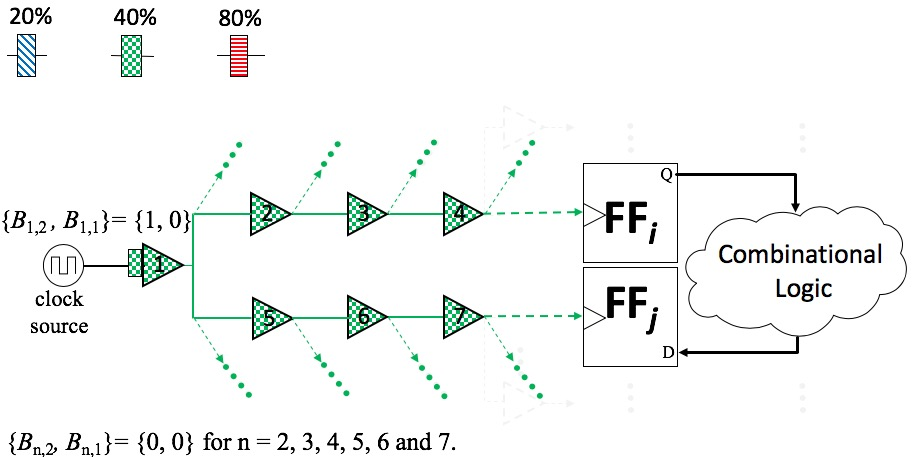
\includegraphics[width=0.92\columnwidth]{A_examlpe_of_DCC_placement1.png}  %IEEE Journal
        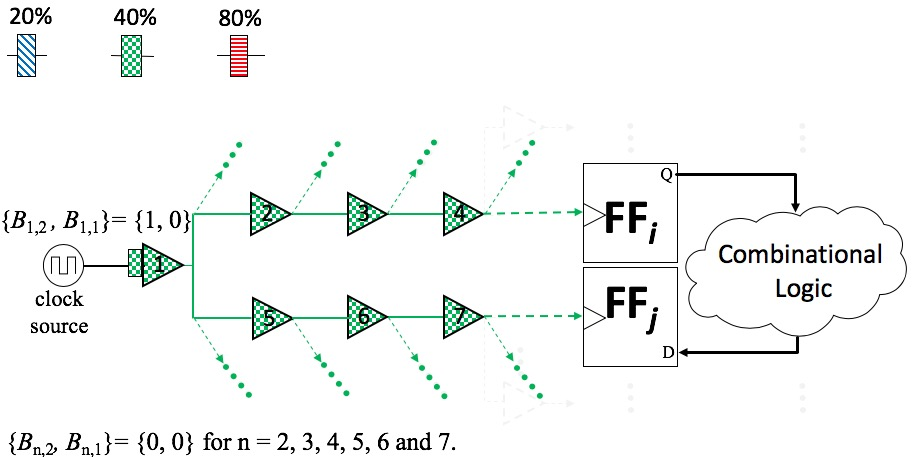
\includegraphics[width=0.65\columnwidth]{A_examlpe_of_DCC_placement1.png}  %ACM Journal
    }
    \hspace{1cm}
    \subfigure[Class 2-2: one DCC on one of the divergent clock paths, or class 3: two DCCs, one on each of the divergent clock paths]{
    	\label{fig:sub:dcci2}
        %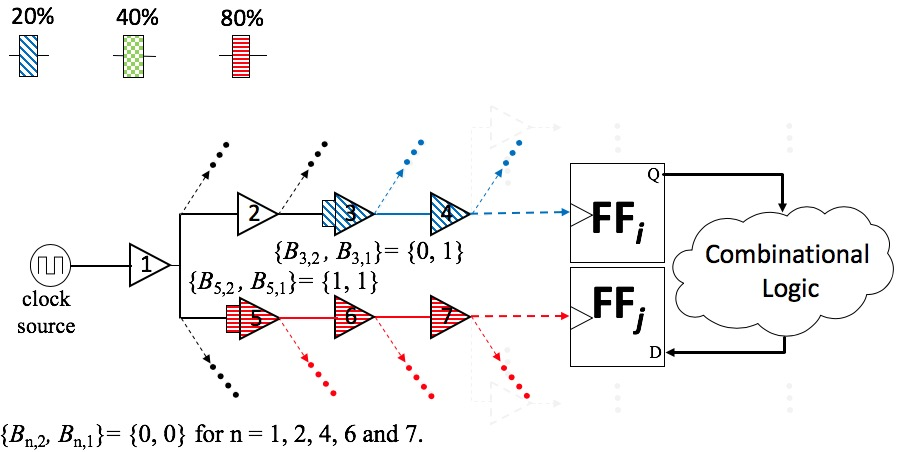
\includegraphics[width=0.92\columnwidth]{A_examlpe_of_DCC_placement2.png}  %IEEE Journal
        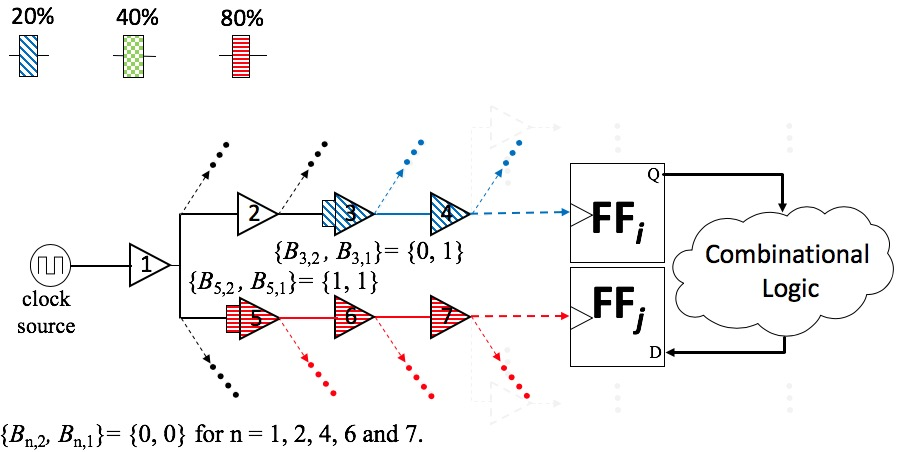
\includegraphics[width=0.65\columnwidth]{A_examlpe_of_DCC_placement2.png}  %ACM Journal
    }
    \caption{Examples of DCC insertion}
    \label{fig:dccinsert}
\end{figure*}
}
